\section{\Large{Бизнес-процесс}}
\addcontentsline{toc}{section}{Бизнес-процесс}

Ниже представлена EPC-диаграмма процесса проведения исследований и
внедрения алгоритмической методики(см. рис\ \ref{pic:analysis__usecases-epc}).

\begin{figure}[H]
	\hspace*{-2.5 cm}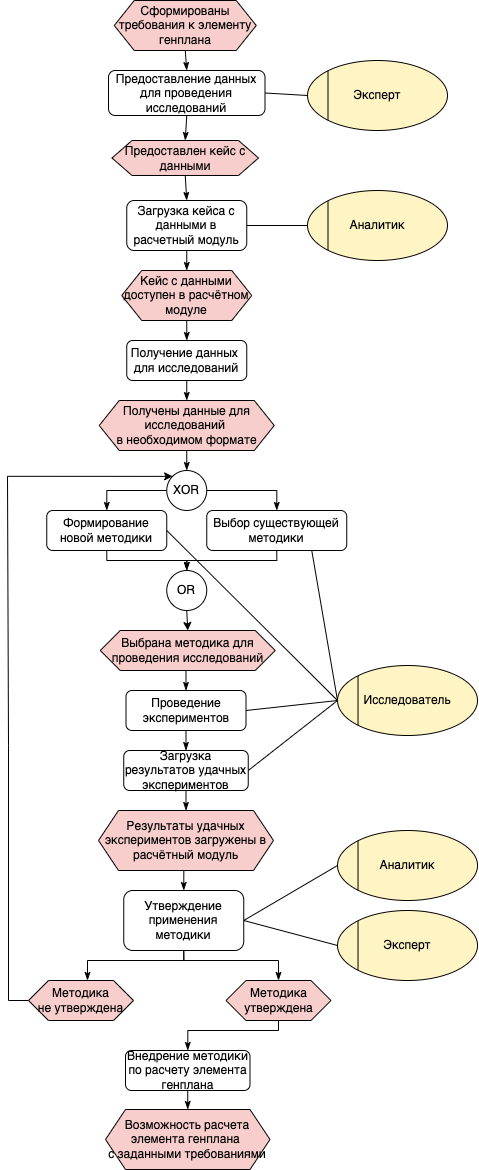
\includegraphics[width=0.55\textwidth, left]{analysis/pictures/usecases/epc}
	\caption{Диаграмма процесса внедрения алгоритмической методики}
	\label{pic:analysis__usecases-epc}
\end{figure}
\vskip 5 mm

Главным инициатором исследований является заказчик. Именно заказчик знает, где найти людей,
обладающих экспертными знаниями в проектировании генеральных планов.
Заказчик так же определяет приоритет появления
новых расчётных элементов на генплане сооружения и количество требований к их размещению.

В любом случае генплан, полученный в автоматическом режиме будет нуждаться в ручной корректировке,
так как в силу очень высокой сложности объектов, невозможно заложить в алгоритмы все требования к формированию.

Процесс обновление алгоритмов выглядит следующим образом.
На первом этапе заказчик решает, требуется ли ему улучшить качество размещения уже существующего элемента
или добавить на генплан новый расчётный элемент.

После этого заказчик сообщает аналитику контактную информацию технического эксперта, с которым может взаимодействовать
аналитик для получения информации по получению презентативных данных для возможности отладки методики
для удовлетворения требований заказчика по размещению объекта генплана.

После получения данных от технического эксперта аналитик оформляет их в виде доступном для загрузки в расчетный модуль.
После того как данные загружены в расчётный модуль, исследователи могут приступать к выработке решения
правильного размещения заданного объекта генерального плана площадного объекта.

У исследователя всегда есть два варианта решения поставленной задачи: создать новую методику решения
или использовать уже существующую.
После того, как сделан выбор, проводится ряд экспериментов,
наиболее удачные результаты экспериментов сохраняются в хранилище и отправляются на анализ аналитику.
Если аналитик принимает решение, что данная методика, позволяет получить решение, соответствующее требованиям
заказчика, то результаты эксперимента уже показываются техническому эксперту со стороны заказчика,
чтобы он дополнительно убедился, что реализация данной методики не противоречит другим требованиям
проектирования генпланов.

Если все хорошо, то методика встраивается в существующее решение. Если же есть какие-то недостатки, то формируется
их набор, где впоследствии они устраняются.
